%!TEX TS-program = xelatex 
%!TEX TS-options = -output-driver="xdvipdfmx -q -E"
%!TEX encoding = UTF-8 Unicode
%
%  summary_5
%
%  Created by Mark Eli Kalderon on 2009-03-04.
%

\documentclass[11pt]{article} 

% Definitions
\newcommand\myauthor{Mark Eli Kalderon} 
\newcommand\mytitle{Oxford Philosophy of Perception:}
\newcommand\mysubtitle{Prichard and the Sense Datum Fallacy}

% Packages
\usepackage{url}
\usepackage{txfonts}
\usepackage{color}
\definecolor{myblue}{rgb}{0.8,0.8,1}

% Define discussion environment
\makeatletter\newenvironment{discussion}{%
   \noindent\begin{lrbox}{\@tempboxa}\begin{minipage}{\columnwidth}\setlength{\parindent}{1em}}{\end{minipage}\end{lrbox}%
   \colorbox{myblue}{\usebox{\@tempboxa}}
}\makeatother

% XeTeX
\usepackage[cm-default]{fontspec}
\usepackage{xltxtra,xunicode}
\defaultfontfeatures{Scale=MatchLowercase,Mapping=tex-text}
\setmainfont{Hoefler Text}
\setsansfont{Gill Sans}
\setmonofont{Inconsolata}

% Title Information
\title{\mytitle\\
\mysubtitle}
\author{\myauthor} 
\date{} % Leave blank for no date, comment out for most recent date

% PDF Stuff
\usepackage[plainpages=false, pdfpagelabels, bookmarksnumbered, backref, pdftitle={\mytitle}, pagebackref, pdfauthor={\myauthor}, xetex, colorlinks=true, linkcolor=gray, urlcolor=gray]{hyperref}

%%% BEGIN DOCUMENT
\begin{document}

% Title Page
\maketitle

% Layout Settings
\setlength{\parindent}{1em}

% Main Content

\begin{figure}[htbp]
    \centering
        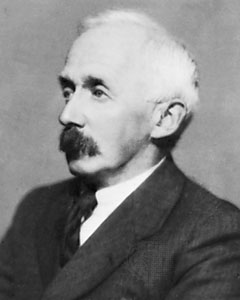
\includegraphics[scale=.5]{../../graphics/prichard.jpg}
    \caption{H.A. Prichard}
    \label{fig:prichard}
\end{figure}

\section{The Theory of Appearing} % (fold)
\label{sec:the_theory_of_appearing}
For Prichard, canonical appearance-attributions take the form:
    \begin{quote}
        \( o \) appears \( F \)
    \end{quote}
An \emph{appearance} is described by a canonical appearance-attribution. Prichard makes five central claims about appearances described by canonical appearance-attributions:
    \begin{enumerate}
        \item Appearance is presentational. An appearance is the presentation of \( o \)---it is \( o \) appearing \( F \) to a subject \( S \).
        \item \( o \) is a body located in space.
        \item The predicate \( F \) has spatial conditions of application---it is intelligibly applied only to spatial bodies.
        \item The spatial body \( o \) is the object of the perception in virtue of which \( o \) appears.
        \item Our perception of \( o \) enables us to apprehend \( o \) and so come to know about it. In Prichard's later terminology, perception is a species of knowledge.
    \end{enumerate}

At least ever since ``Seeing Movement'' written in 1921, Prichard abandons the theory of appearing. Specifically:
        \begin{enumerate}
            \item He denies that bodies are the object of perception.
            \item He denies that perception is a species of knowledge.
        \end{enumerate}
% section the_theory_of_appearing (end)

\section{Perception as a Species of Knowledge} % (fold)
\label{sec:perception_as_a_species_of_knowledge}
While Prichard primarily casts his discussion in terms of \emph{knowledge}, various writers are held to be committed to the thesis that perception is a species of knowledge if in perceiving something the subject \emph{apprehends} it, is \emph{conscious} of it, or is \emph{aware} of it. There are important differences between these notions. Prichard is evidently thinking of knowledge as a genus of which these different attitudes are species.

\begin{discussion}
    Craig French wondered whether this really made sense. Normally, we think that perception affords awareness of things in our environment and this puts us in a position to know about these things. So understood, awareness is distinct from knowledge. Indeed, while knowledge takes a propositional object, awareness need not. 
    
    If Prichard's coherent, we must understand knowledge, as he understands it, in a more expansive sense. It is the most general category of certain kind of cognitive attitudes (cognitive in the sense that contrasts with connative and not in the sense that these attitudes are analyzable or otherwise reducible to beliefs.) This kind of cognitive attitude takes either propositional or nonpropositional objects. The relevant propositional attitudes are all \emph{factive}. The nonpropositional attitudes are all object involving in the sense that one can only have that attitude toward an object if that object exists.
\end{discussion}

The theory of appearing was a theoretical development of Cook Wilson's reflections on the nature of appearance. While Prichard abandons the theory of appearance, he retains, throughout his career, Cook Wilson's conception of knowledge. One feature of this conception is presently important:
\begin{quote}
    The object of knowledge is independent of the act of knowing.
\end{quote}
To maintain, then, that perception is a species of knowledge is to maintain that the object of perception is independent of the subject's perceiving it. Prichard's opposition to the idea that perception is a species of knowledge is motivated by the Berkelean contention that the objects of perception are dependent on perceiving them.
% section perception_as_a_species_of_knowledge (end)

\section{The Structure of the Sense Datum Falacy} % (fold)
\label{sec:the_structure_of_the_sense_datum_falacy}
``The Sense Datum Fallacy'' falls into four parts:
\begin{enumerate}
    \item The first part introduces the theme of the paper. (1-3)
    \item The second part argues that a familyt of anti-idealist arguments belonging to a tradition inagurated by Moore all turn on the thesis that perception is a species of knowledge. (4-7)
    \item The third part argues against the thesis that perception is a species of knowledge. (7-12)
    \item The fourth part argues that the sense datum theory is committed to the problematic thesis that perception is a species of knowledge. (12-18)
\end{enumerate}
% section the_structure_of_the_sense_datum_falacy (end)

\section{Introduction} % (fold)
\label{sec:introduction}
Prichard begins by considering two questions:
\begin{enumerate}
    \item What are the objects of peception?
    \item Do the objects of perception depend on the subject's perceiving them?
\end{enumerate}
And he contrasts the naïve realist's answer with Berkeley's.

According to the naïve realist:
\begin{enumerate}
    \item The objects of perception are bodies.
    \item Bodies are not dependent on our perceiving them.
\end{enumerate}
(Indeed, Prichard thinks that it is part of the meaning of ``body'' that a body is independent f our perception of it. So understood, ``external body'' is redundant.)

Berkeley in contrast maintains that:
\begin{enumerate}
    \item a. The objects of perception are secondary qualities. b. These have a ``common character''---they are sensations.
    \item Given the nature of sensations, they are dependent on a subject's perceiving them.
\end{enumerate}

Prichard observes that contemporary writers agree with Berkeley that the object's of perception are secondary qualities. But they maintain, instead, that these are sense data. And as a consequence, certain questions arise about the nature of sense data, that do not arise if secondary qualities are understood as sensations. Moreover, the substitution of sense data for sensations is fallacious in the sense that it depends on the false thesis that perception is a species of knowledge.

A couple of comments:
\begin{enumerate}
    \item This is not really a fallacy. Prichard is not charging the sense data theorist with \emph{invalid} reasoning so much as \emph{unsound} reasoning.
    \item Prichard is emphasizing certain hard metaphysical questions about the nature of sense data that seem not to admit of determinate answers. In this way he is echoing G.A. Paul's worries about the persistence-conditions of sense data. However, whereas Paul maintains that these embarassing questions only arise f the existence of sense data is regarded as a substantive metaphysical issue, Prichard seems not to consider the idea advocated by Paul and Ayer that the existence of sense data is not a substantive metaphysical issue.

\section{The Anti-Idealist Arguments of Kemp Smith and Moore} % (fold)
\label{sec:the_anti_idealist_arguments_of_kemp_smith_and_moore}
Kemp Smith's argument:
\begin{enumerate}
    \item The objects of perception are secondary qualities.
    \item Secondary qualities are sensations.
    \item However, what Berkely fails to notice is that sensation is ambiguous. A sensation may either be:
    \begin{enumerate}
        \item the object apprehended, or
        \item the act of apprehension
    \end{enumerate}
    \item The claim that secondary qualities are sensations is only true of sensations are understood as the objects of apprehension.
    \item Berkely thus fallaciously reasons from our perceiving sensations to tehese being dependent on our perceiving them. The subjective idealist claim only follows on the other reading of sensation. But so understood the claim is false.
    \item Further, if sensations are the objects of apprehension, then they are not dependent on our apprehension of them in perception.
\end{enumerate}

Both Moore's and Kemp Smith's arguments crucially depend on the thesis that perception is a species of knowledge. In Kemp Smith's argument, this is manifest in his claim that in seeing a color, the color is the object of apprehension.
% section the_anti_idealist_arguments_of_kemp_smith_and_moore (end)
\end{enumerate}

\section{Why Perception is Not a Species of Knowledge} % (fold)
\label{sec:why_perception_is_not_a_species_of_knowledge}
Prichard gives three arguments:
\begin{enumerate}
    \item The supposition that the objects of perception existe independently of our perceiving them raises substantive metaphysical questions that admit of no determinate answers.
    \item The secondary qualities that we perceive depend on our perception of them and so perception is not a species of knowledge.
    \item If perceiving were a kind of knowing, mistakes would not be possible, but they are.
\end{enumerate}

\begin{enumerate}
    \item Suppose that Berkeley is right that the objects of perception are secondary qualities. But suppose that, contrary to Berkeley, perception is a species of knowledge. Then secondary qualities would exist independently of our perceiving them. But now, certain questions arise about the nature of these secondary qualities. Specifically questions about their publicity, persistence-conditions, their material or mental nature, and their causal origin. Kemp Smith accepts that these are substantive metaphysical questions but concedes that they admit of no determinate answers. Prichard insinuates, however, that if sense data really do exist, then there would be determinate answers to these questions.
    \begin{discussion}
        Craig French wondered whether we should accept the claim that if sense data exist, then there are determinate answers to these metaphysical questions. There is no verificationist thought at work in the background as their might be with Ayer. I suspect that Prichard's argument here is meant to be nondemonstrative---the best explanation for why we lack determinate answers concerning the nature of sense data is that there are no such things.
    \end{discussion}
    \item Berekely and his modern opposnents are right in thinking that what we perceive in each kind of perception is an appropriate kind of secondary quality. Berkely however is right that the secondary qualities depend on our perception of them. Prichard supports this by asking us to consider the case of audition. Berkeley's claim that sounds are the primary objects of auditory experience is plausible. But even conceding this much to Berkeley seems not to ibviously commit us to sounds being dependent upon our hearing them
\end{enumerate}
% section why_perception_is_not_a_species_of_knowledge (end)
% section introduction (end)

\end{document}
